\chapter[Metodologia]{Metodologia}
\label{cap:metodologia}

Neste capítulo, são descritos os procedimentos científicos e experimentais empregados no desenvolvimento do RECLin-PT, incluindo o procedimento comum de ajuste fino de \emph{encoders} pré-treinados, o \emph{dataset} utilizado, a preparação do ambiente
experimental, as métricas de avaliação, a preparação dos dados e o protocolo que
rege a seleção e a comparação dos modelos. O funcionamento do RECLin-PT, isto é, sua
arquitetura e as estratégias investigadas, é apresentado no
Capítulo~\ref{cap:prototipo}. Os procedimentos descritos aqui são o instrumento pelo
qual as decisões de modelagem do RECLin-PT, a escolha do \emph{encoder} e da
estratégia, passam a se apoiar em evidência medida, e não em preferência prévia.
Todas as etapas foram projetadas com foco na reprodutibilidade. Para isso, os artefatos são identificados por \emph{hashes}, e as decisões tomadas sobre os dados são registradas antes de sua utilização.

\section{\emph{Fine-tuning} de \emph{encoders} pré-treinados}
\label{sec:finetuning}

Os modelos deste trabalho partem de \emph{encoders} pré-treinados, redes da família BERT \cite{devlin_2019_bert} que já aprenderam, sobre grandes volumes de texto
não anotado, a produzir uma representação vetorial contextual para cada
\emph{token}. Esse conhecimento prévio é a razão de usá-los. Em vez de aprender a
língua a partir dos poucos exemplos anotados da tarefa, o modelo parte de pesos que
já codificam vocabulário, morfologia e relações sintáticas, e o treino só precisa
especializá-los. O \emph{encoder} é escolhido a partir de seu \emph{checkpoint} de pré-treinamento. Neste trabalho, são considerados o BioBERTpt-all e o BioBERTpt-clin, ambos de domínio clínico, e o BERTimbau-base, de domínio geral (Seção~\ref{sec:encoders}).

O \emph{fine-tuning} (ajuste fino) adapta esses pesos à extração de relações.
Cada exemplo é um par de entidades, apresentado ao modelo como uma janela de texto em
torno do par, com as duas entidades delimitadas por marcadores
(Seção~\ref{sec:markers}). O \emph{encoder} transforma a janela em representações contextuais, enquanto uma cabeça de classificação, composta por uma nova camada adicionada sobre ele, converte essas representações em uma pontuação para cada rótulo. Durante o
treino, as predições são comparadas aos rótulos anotados por uma função de perda de
entropia cruzada. O gradiente dessa perda é propagado de volta por toda a rede
(retropropagação), e um otimizador atualiza tanto a cabeça quanto os pesos do
\emph{encoder}. Como as classes são muito desbalanceadas, a perda de cada exemplo é
ponderada pelo inverso da frequência de sua classe no treino, com peso
$n/(K\cdot n_c)$, em que $n$ é o número de exemplos, $K$ o número de classes e $n_c$
o número de exemplos da classe $c$. Sem essa ponderação, o modelo minimizaria o erro
prevendo \texttt{no\_relation} para quase tudo.

O procedimento de treino é o mesmo para todas as estratégias treinadas e segue a
configuração do Quadro~\ref{quad:hiperparametros}. Os exemplos de treino são
apresentados em lotes de 64, embaralhados por um gerador com semente fixa. O
otimizador é o AdamW, com taxa de aprendizado de $2\times10^{-5}$ e
\emph{weight decay} de $0{,}01$. A taxa cresce linearmente durante os primeiros 10\%
dos passos (aquecimento) e decresce linearmente até zero, e a norma do gradiente é
limitada a 1. O treino percorre um número fixo de épocas, sem parada
antecipada. Ao fim de cada época, o modelo é avaliado no conjunto de desenvolvimento
(DEV) pelo critério da estratégia, e os pesos da melhor época são restaurados ao
final. Essa é a única escolha feita durante o treino, e ela usa apenas o DEV
(Seção~\ref{sec:protocolo}). Para que a mesma configuração produza os mesmos números
no mesmo ambiente, as sementes de Python, NumPy e PyTorch são fixadas, as operações
determinísticas da GPU são exigidas sempre que disponíveis, e o estado completo dos
geradores aleatórios é salvo nos \emph{checkpoints}, o que permite retomar um treino
interrompido exatamente do ponto em que parou.

\begin{quadro}[htbp]
  \centering
  \caption{Hiperparâmetros e configuração do \emph{fine-tuning}, comuns às estratégias treinadas.}
  \label{quad:hiperparametros}
  \small
  \begin{tabular}{l >{\raggedright\arraybackslash}p{8.8cm}}
  \toprule
  Item & Valor \\
  \midrule
  Entrada & janela de $\pm128$ caracteres em torno do par (\texttt{ctx\_chars}), com marcadores \texttt{[E1]}/\texttt{[E2]}, sem tipo semântico; até 128 \emph{tokens} (\texttt{max\_length}) \\
  Pares candidatos & distância máxima de 25 caracteres entre as entidades (\texttt{max\_gap}) \\
  Lote (\emph{batch}) & 64 \\
  Otimizador & AdamW; taxa de aprendizado $2\times10^{-5}$; \emph{weight decay} $0{,}01$ \\
  Escalonador & linear, com aquecimento nos primeiros 10\% dos passos \\
  Norma máxima do gradiente & 1,0 \\
  Perda & entropia cruzada ponderada (\texttt{class\_weight="balanced"}), com pesos calculados no treino de cada estratégia ou estágio \\
  Épocas & 3 (estratégias de três rótulos e estágio 1 do Two-Stage); 10 (estágio 2) \\
  Seleção da época & maior macro-F1 no DEV (estratégias de três rótulos); critérios próprios nos estágios do Two-Stage \\
  Semente & 42 \\
  \bottomrule
  \end{tabular}\\[4pt]
  {\footnotesize Fonte: elaborado pelo autor.}
\end{quadro}

O \emph{fine-tuning} é a base comum de todas as estratégias treinadas, que diferem na
forma de ler a representação do \emph{encoder} e de organizar a decisão. Duas
estratégias apenas pós-processam as predições do baseline, sem treino próprio. A
distinção entre \emph{encoder}, estratégia e modelo RECLin-PT, assim como a descrição
de cada estratégia, está no Capítulo~\ref{cap:prototipo}.

\section{O \emph{dataset} SemClinBr}
\label{sec:corpus}

Os documentos clínicos utilizados neste trabalho foram retirados do
\textbf{SemClinBr} \cite{oliveira_2022_semclinbr}\footnote{Repositório do corpus e
formulário de requisição de acesso em
\href{https://github.com/HAILab-PUCPR/SemClinBr}{github.com/HAILab-PUCPR/SemClinBr}.},
primeiro corpus clínico em português do Brasil anotado semanticamente. Ele reúne mil
documentos provenientes de múltiplas instituições e especialidades, redigidos por
profissionais de saúde no registro do cuidado, e é distribuído mediante solicitação
formal, para uso não comercial. Neste trabalho, o SemClinBr é a única fonte de dados:
dele saem os exemplos de treino, a escolha de modelos no DEV e o conjunto de teste
reservado para a avaliação final.

O texto do corpus é típico do prontuário. As frases são curtas e telegráficas, com
omissão de verbos e artigos, abreviações frequentes e não padronizadas (como MSE,
para membro superior esquerdo), mistura de letras maiúsculas e minúsculas e ausência
ocasional de acentos, e construções negativas recorrentes, como ``sem sinais
flogísticos'' ou ``nega queixas''. Essas características afastam o texto da
linguagem dos corpora usados no pré-treino de domínio geral e motivam a comparação
entre \emph{encoders}.

Cada documento traz anotações de entidades, trechos do texto delimitados
por posições de caractere (\emph{offsets}) e associados a tipos semânticos da UMLS,
além de categorias próprias como \texttt{Abbreviation} e \texttt{Negation}. Uma
mesma entidade pode receber vários tipos, separados por ``|''. Entre as entidades,
são anotadas relações dirigidas, de um primeiro argumento ($e_1$) para um
segundo ($e_2$), de dois tipos: \texttt{associated\_with}, que liga conceitos
relacionados, como um dispositivo e a região do corpo em que está, e
\texttt{negation\_of}, que liga uma expressão de negação ao conceito negado. A
\autoref{fig:exemplo_anotacao} mostra um trecho real de um documento do corpus, com
as entidades e as relações anotadas.

% Exemplo real de anotação do SemClinBr: documento 9091 (partição de treino),
% offsets 1060--1127. Texto, entidades (id, tipo) e relações conferidos no XML
% original (9091.xml) e nos dados derivados (particoes, train.jsonl): idênticos.
\begin{figure}[htbp]
  \centering
  \caption{Exemplo real de anotação de um documento do SemClinBr (documento 9091, trecho): entidades anotadas, com seus identificadores, e relações entre elas.}
  \label{fig:exemplo_anotacao}
  \begin{tikzpicture}[
      font=\sffamily\small,
      ent/.style={draw=black!70, fill=black!6, rounded corners=2pt, inner xsep=2.5pt, inner ysep=3pt, anchor=base west},
      neg/.style={draw=black!70, fill=black!18, rounded corners=2pt, inner xsep=2.5pt, inner ysep=3pt, anchor=base west},
      txt/.style={inner xsep=1.2pt, inner ysep=3pt, anchor=base west},
      ident/.style={font=\sffamily\scriptsize, text=black!65, below=1pt},
      relneg/.style={-{Stealth[length=2.2mm]}, line width=1.1pt, draw=black},
      relass/.style={-{Stealth[length=2.2mm]}, line width=0.7pt, draw=black!60, dashed},
      rot/.style={font=\sffamily\scriptsize, fill=white, inner sep=1pt}
    ]
    \node[ent] (a) at (0,0) {acesso venoso periferico};
    \node[txt] (t1) at ([xshift=0.6mm]a.base east) {em};
    \node[ent] (b) at ([xshift=0.6mm]t1.base east) {MSE};
    \node[neg] (c) at ([xshift=1.4mm]b.base east) {sem};
    \node[ent] (d) at ([xshift=1.4mm]c.base east) {sinais flogisticos};
    \node[txt] (t2) at ([xshift=0.6mm]d.base east) {e};
    \node[ent] (e) at ([xshift=0.6mm]t2.base east) {salinizado};
    \node[ident] at (a.south) {9553};
    \node[ident] at (b.south) {9513};
    \node[ident] at (c.south) {9514};
    \node[ident] at (d.south) {9554};
    \node[ident] at (e.south) {9515};
    % relações (e1 -> e2, como anotadas)
    \draw[relass] ([xshift=-1mm]b.north) .. controls +(0,0.75) and +(0,0.75) .. ([xshift=-6mm]a.north)
      node[rot, pos=0.5, above=-1pt] {associated\_with};
    \draw[relneg] (c.north) .. controls +(0,0.75) and +(0,0.75) .. ([xshift=-4mm]d.north)
      node[rot, pos=0.5, above=-1pt] {negation\_of};
    \draw[relass] ([xshift=4mm]d.north) .. controls +(0,1.55) and +(0,1.55) .. (a.north)
      node[rot, pos=0.5, above=-1pt] {associated\_with};
    \draw[relass] (e.north) .. controls +(0,2.35) and +(0,2.35) .. ([xshift=6mm]a.north)
      node[rot, pos=0.5, above=-1pt] {associated\_with};
  \end{tikzpicture}\\[6pt]
  {\footnotesize
  \begin{tabular}{lll}
  \toprule
  Id & Entidade & Tipo anotado \\
  \midrule
  9553 & acesso venoso periferico & \emph{Therapeutic or Preventive Procedure}$|$\emph{Medical Device} \\
  9513 & MSE & \emph{Body Location or Region}$|$\emph{Abbreviation} \\
  9514 & sem & \emph{Negation} \\
  9554 & sinais flogisticos & \emph{Sign or Symptom} \\
  9515 & salinizado & \emph{Therapeutic or Preventive Procedure}$|$\emph{Finding} \\
  \bottomrule
  \end{tabular}}\\[4pt]
  {\footnotesize Fonte: elaborado pelo autor a partir de dados do SemClinBr \cite{oliveira_2022_semclinbr}.}
\end{figure}


No trecho, a entidade ``sem'' (tipo \texttt{Negation}) é o primeiro argumento de uma
relação \texttt{negation\_of} cujo segundo argumento é ``sinais flogisticos'': o
registro afirma a \emph{ausência} de sinais inflamatórios no acesso venoso, e um
sistema que perdesse essa relação leria o achado como presente. As outras três
relações, do tipo \texttt{associated\_with}, ligam a localização (``MSE''), o achado
negado e o estado (``salinizado'') ao dispositivo descrito.

Três características da anotação afetam diretamente o treino e a avaliação. A
primeira é o desbalanceamento: das $11\,458$ relações anotadas no corpus,
$9\,852$ são \texttt{associated\_with} e apenas $1\,606$ ($14{,}02\%$) são
\texttt{negation\_of}. A segunda é que o corpus anota apenas relações
positivas. Um par de entidades sem anotação não é, por si, um exemplo explícito de
ausência de relação, e por isso os exemplos negativos (\texttt{no\_relation}) precisam
ser construídos a partir dos pares não anotados (Seção~\ref{sec:candidatos}), o que
agrava ainda mais o desbalanceamento. A terceira é que as relações são
dirigidas: o par $(e_1, e_2)$ e o par inverso são exemplos diferentes, e só um deles
pode carregar a relação anotada.

\section{Preparação do ambiente}
\label{sec:ambiente}

Os experimentos foram organizados em um pacote Python próprio, versionado em um
repositório Git\footnote{Código e resultados em
\href{https://github.com/angeloalsf/RECLin-PT}{github.com/angeloalsf/RECLin-PT}
(branch \texttt{resultados-colab}). O corpus SemClinBr não é redistribuído, por ter
acesso restrito.}, que reúne a leitura do corpus, as partições, a geração de
candidatos, as estratégias, o treino, a avaliação e os relatórios. O
Quadro~\ref{quad:ambiente} resume os ambientes utilizados e as versões registradas
pelo próprio código em cada execução.

\begin{quadro}[htbp]
  \centering
  \caption{Ambientes de execução e versões das principais bibliotecas.}
  \label{quad:ambiente}
  \small
  \begin{tabular}{l >{\raggedright\arraybackslash}p{9.4cm}}
  \toprule
  Item & Valor \\
  \midrule
  Treino e avaliação no DEV & Google Colab, GPU NVIDIA Tesla T4 (15 GB), CUDA 13.0 \\
  Python & 3.13 (treino); 3.10 (reconstrução dos dados, no computador do autor) \\
  Bibliotecas & PyTorch 2.11.0, Transformers 5.16.1, Tokenizers 0.23.2, Hugging Face Hub 1.29.0, Safetensors 0.8.0, NumPy 2.1.3, SciPy 1.16.3 \\
  Pesos pré-treinados & \texttt{pucpr/biobertpt-all} (revisão \texttt{36b11cf}) e \texttt{neuralmind/\allowbreak bert-base-portuguese-cased} (revisão \texttt{94d69c9}), baixados por revisão exata e conferidos por \emph{hash} \\
  Determinismo & \texttt{PYTHONHASHSEED=0}, \texttt{CUBLAS\_WORKSPACE\_CONFIG=:4096:8}, sementes fixas e algoritmos determinísticos do PyTorch \\
  \bottomrule
  \end{tabular}\\[4pt]
  {\footnotesize Fonte: elaborado pelo autor.}
\end{quadro}

A reconstrução dos dados a partir dos XML do corpus foi executada no
computador do autor, porque os arquivos originais não podem ser redistribuídos. O
resultado são partições derivadas, identificadas por \emph{hashes}
(Seção~\ref{sec:preparacao}). O treino foi executado no Google Colab, com
um \emph{notebook} por estratégia, que obtém o código do repositório, confere o
ambiente e a GPU e chama os \emph{scripts} de treino. Os pesos pré-treinados são
baixados uma única vez, na revisão exata registrada no protocolo, e carregados sem
acesso à rede, com os \emph{hashes} de todos os arquivos conferidos antes de cada
carga. As versões das bibliotecas são fixadas por um arquivo de restrições, com o
qual o pacote é instalado.

Cada execução grava uma pasta própria com a configuração completa
(\texttt{config.json}), o histórico de treino por época e as sessões
(\texttt{treino.json}), as métricas (\texttt{metricas.json}), as predições do DEV
(\texttt{predicoes\_dev.json}) e o registro do ambiente e da proveniência
(\texttt{experimento.json}). Os \emph{checkpoints}, que permitem retomar um treino
interrompido, são espelhados no Google Drive durante o treino. Para reproduzir os
experimentos, basta instalar o pacote com as versões fixadas, conferir as partições
contra o manifesto e executar os \emph{scripts} de treino com a mesma configuração e
semente. As tabelas e figuras deste trabalho são regeneradas a partir das pastas das
execuções por \emph{scripts}, sem transcrição manual de números.

\section{Métricas utilizadas para avaliar os modelos}
\label{sec:metricas}

Nesta seção são apresentadas as métricas utilizadas para avaliar o desempenho dos
modelos de extração de relações. As métricas centrais são a precisão
(\emph{precision}), o \emph{recall} e o F1-\emph{Score}, calculadas para cada uma das
três classes da tarefa, \texttt{negation\_of}, \texttt{associated\_with} e
\texttt{no\_relation}. Para uma classe, um par conta como verdadeiro positivo (TP)
quando é dessa classe e o modelo o atribui a ela; como falso positivo (FP) quando o
modelo o atribui à classe sem que ele pertença a ela; e como falso negativo (FN)
quando pertence à classe e o modelo o atribui a outra.

A precisão (\emph{precision}) é calculada pela razão entre o número de verdadeiros
positivos e o total de previsões positivas realizadas pelo modelo. Essa métrica indica
a proporção de previsões positivas que foram classificadas corretamente, conforme
apresentado na Fórmula~\ref{eq:precisao}.

\formula{Precisão}{eq:precisao}
\[
  \text{Precisão} =
  \frac{\text{Verdadeiros positivos}}
       {\text{Verdadeiros positivos} + \text{Falsos positivos}}
\]

O \emph{recall}, também conhecido como sensibilidade ou taxa de detecção, corresponde
à proporção de exemplos positivos reais que foram identificados corretamente pelo
modelo. Dessa forma, a métrica permite avaliar a capacidade do modelo de recuperar os
exemplos pertencentes à classe analisada, conforme apresentado na
Fórmula~\ref{eq:recall}.

\formula{\emph{Recall}}{eq:recall}
\[
  \text{\emph{Recall}} =
  \frac{\text{Verdadeiros positivos}}
       {\text{Verdadeiros positivos} + \text{Falsos negativos}}
\]

Por fim, o F1-\emph{Score} combina as medidas de precisão e \emph{recall} por meio da
média harmônica entre elas. Essa métrica permite avaliar conjuntamente a capacidade do
modelo de realizar previsões positivas corretas e identificar os exemplos positivos
reais. Seu cálculo é apresentado na Fórmula~\ref{eq:f1}.

\formula{F1-\emph{Score}}{eq:f1}
\[
  \text{F1-\emph{Score}} =
  2 \cdot \frac{\text{Precisão} \cdot \text{\emph{Recall}}}
               {\text{Precisão} + \text{\emph{Recall}}}
\]

No código do projeto, as três métricas são calculadas a partir da matriz de confusão,
com o F1 na forma equivalente $2\,TP/(2\,TP + FP + FN)$, e valem zero quando o
denominador é nulo, por exemplo quando o modelo nunca prediz a classe. O F1 de
\texttt{negation\_of} é a métrica primária do trabalho. Para resumir o
desempenho nas três classes, usa-se o macro-F1, média simples dos três F1,
que dá o mesmo peso a cada classe e, por isso, penaliza modelos que negligenciam as
minoritárias \cite{forman_2010_apples}. Ele é também o critério de seleção de época
das estratégias de três rótulos. São reportados ainda a acurácia, pouco informativa
isoladamente porque \texttt{no\_relation} domina os pares, e o coeficiente de
correlação de Matthews (MCC) multiclasse, que considera a matriz de confusão inteira e
é robusto ao desbalanceamento.

\section{Preparação dos dados}
\label{sec:preparacao}

\subsection{Reconstrução dos dados e alinhamento dos offsets}
\label{sec:parsing}

Os dados empregados foram reconstruídos diretamente dos XML do SemClinBr. Um
\emph{parser} lê cada arquivo e produz um registro com identificador do documento,
texto, entidades (tipo e offsets) e relações, sem normalizar tipos e sem alterar ou
descartar nenhuma anotação. O ponto crítico da reconstrução é o alinhamento entre o
texto e os offsets. Em parte dos documentos, os offsets foram calculados sobre o texto
com quebras de linha de dois caracteres, e substituir cada quebra por um único espaço
desloca todas as entidades seguintes. A regra adotada identifica, por documento e com
todas as anotações, qual convenção os offsets seguem e, quando é a de dois caracteres,
substitui cada quebra por dois espaços, de modo que o texto passe a ter o comprimento
pressuposto pelos offsets. A regra transformou 421 dos 1.000 documentos. Nos demais, o
texto foi mantido sem alteração.

O resultado foi verificado por auditoria: nenhuma entidade das três partições
apresenta divergência entre o trecho recortado pelo offset e o texto anotado, e a
reconstrução preserva os documentos de cada partição, as entidades, as relações, os
pares candidatos e os rótulos de referência. As 26 anomalias de anotação encontradas
(por exemplo, um offset inválido) foram mantidas como estão e registradas em arquivo
próprio. Um manifesto (\texttt{MANIFEST.json}) registra o SHA-256 de cada partição,
as contagens e a proveniência da fonte (Apêndice~\ref{ap:sha256}).

\subsection{Caracterização do corpus}
\label{sec:eda}

A análise exploratória (\foreignlanguage{english}{Exploratory Data Analysis}, EDA)
foi conduzida com as próprias funções do código do projeto, totalizando $1\,000$
documentos, $45\,508$ entidades e $11\,458$ relações. A mediana é de $10$ relações por
documento, o percentil 90 é de $24$ e o máximo é de $65$; $46$ documentos não possuem
relação anotada. Entre as categorias de entidade, contadas como ocorrências do
rótulo depois de decompor as anotações multirrótulo, predominam
\texttt{Abbreviation} ($12\,592$), \texttt{Finding} ($6\,827$) e
\texttt{Therapeutic or Preventive Procedure} ($4\,759$), e a categoria
\texttt{Negation} soma $2\,646$ ocorrências. Como a anotação de uma mesma entidade
pode repetir um rótulo, essas contagens superam o número de entidades com cada tipo:
são $12\,290$, $6\,747$, $4\,716$ e $2\,299$ entidades, respectivamente. Os
controles da Seção~\ref{sec:controles_tipo} contam entidades, e não ocorrências do
rótulo.

A Tabela~\ref{tab:distancia} e a \autoref{fig:eda_dist} mostram que as relações
ocorrem entre entidades próximas, com um contraste nítido entre os tipos. A negação é
praticamente adjacente, com mediana e percentil 75 de um único caractere, enquanto a
associação se distribui por uma cauda bem mais longa. Essa assimetria fundamenta a
janela máxima (\texttt{max\_gap}$=25$) da geração de pares candidatos
(Seção~\ref{sec:teto_recall}). A análise de distâncias usou as relações \emph{gold}
do corpus completo, inclusive as das partições de desenvolvimento e de teste.
\label{sec:eda_distancia}

%% GERADO por analise/gerar_artefatos_tcc.py -- nao edite a mao.
\begin{table}[htbp]
  \centering
  \caption{Distância em caracteres entre as entidades de cada relação anotada (corpus completo).}
  \label{tab:distancia}
  \begin{tabular}{lrrrrrrr}
  \toprule
  Tipo & $n$ & Média & Mediana & p75 & p95 & Máx. & $>25$ \\
  \midrule
\texttt{negation\_of} & 1\,606 & 3{,}5 & 1 & 1 & 15 & 54 & 1{,}87\% \\
\texttt{associated\_with} & 9\,852 & 11{,}8 & 4 & 10 & 43 & 541 & 9{,}89\% \\
  \bottomrule
  \end{tabular}\\[4pt]
  {\footnotesize Fonte: elaborado pelo autor.}
\end{table}


\begin{figure}[htbp]
  \centering
  \caption{Distribuição da distância em caracteres entre entidades relacionadas (recorte em 200), com a janela \texttt{max\_gap} assinalada.}
  \label{fig:eda_dist}
  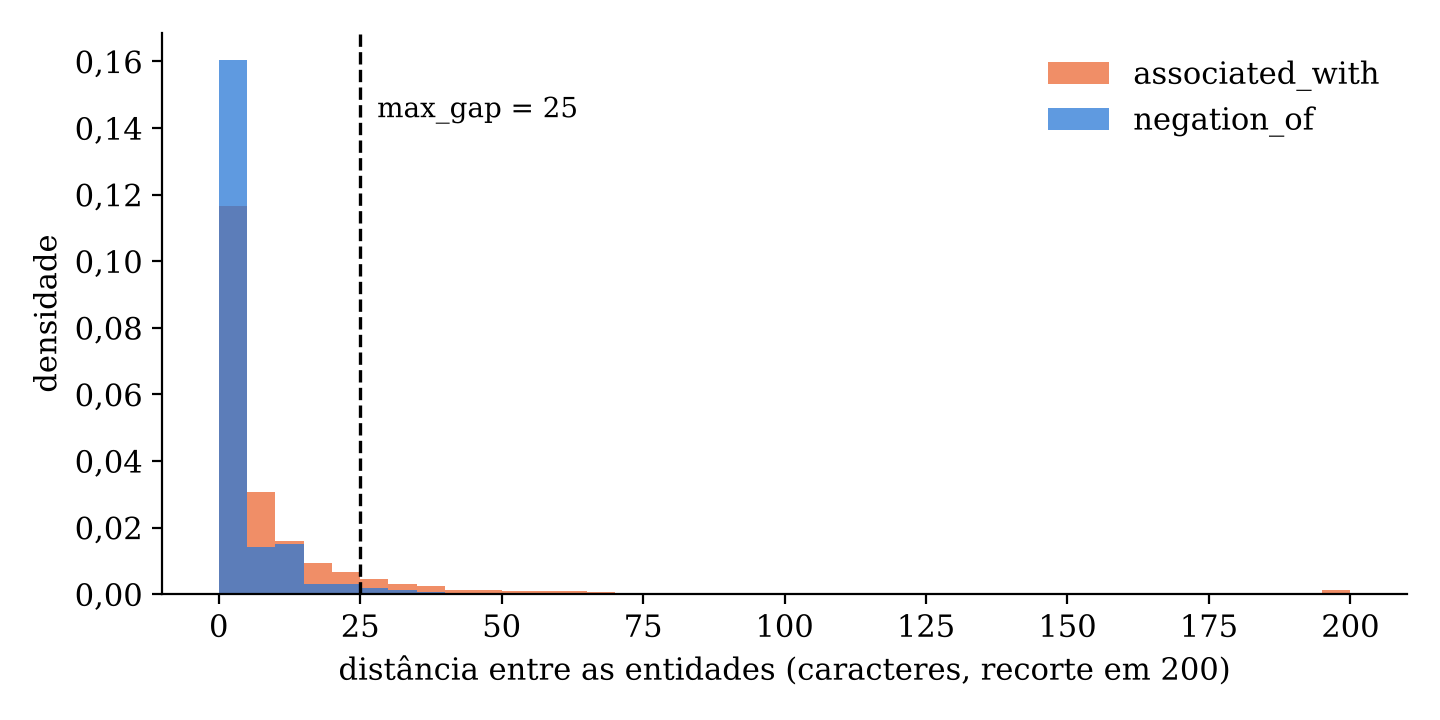
\includegraphics[width=0.8\textwidth]{resultados/eda_distancia.png}\\[4pt]
  {\footnotesize Fonte: elaborado pelo autor.}
\end{figure}

\subsection{Particionamento dos dados}
\label{sec:particao}

A partição segue a razão 80/10/10 em nível de documento, e não de relação.
Essa escolha previne o vazamento de dados, pois relações de um mesmo documento
compartilham vocabulário e trechos repetidos, e dividi-las entre partições inflaria
artificialmente as métricas. A partição é estratificada pela presença de
\texttt{negation\_of}: os documentos com ao menos uma relação de negação e os demais
são embaralhados separadamente, com semente $42$, e divididos 80/10/10 dentro de cada
grupo, o que garante exemplos da classe rara nas três partições. O resultado são
$800$ documentos de treino, $100$ de DEV e $100$ de teste, congelados e verificados
por SHA-256 (Apêndice~\ref{ap:sha256}). A Tabela~\ref{tab:corpus} apresenta as
contagens por partição.

%% GERADO por analise/gerar_artefatos_tcc.py -- nao edite a mao.
\begin{table}[htbp]
  \centering
  \caption{Partições congeladas: documentos, entidades, relações anotadas e pares candidatos (\texttt{max\_gap}$=25$).}
  \label{tab:corpus}
\resizebox{\textwidth}{!}{%
  \begin{tabular}{lrrrrrr}
  \toprule
  Partição & Documentos & Entidades & \texttt{negation\_of} & \texttt{associated\_with} & Candidatos & \texttt{no\_relation} \\
  \midrule
Treino & 800 & 36\,455 & 1\,299 & 7\,922 & 152\,686 & 144\,335 \\
Desenvolvimento & 100 & 4\,513 & 155 & 832 & 19\,064 & 18\,151 \\
Teste & 100 & 4\,540 & 152 & 1\,098 & 19\,210 & 18\,062 \\
\midrule
Total & 1\,000 & 45\,508 & 1\,606 & 9\,852 & 190\,960 & 180\,548 \\
  \bottomrule
  \end{tabular}}\\[4pt]
  {\footnotesize Fonte: elaborado pelo autor.}
\end{table}


Trata-se de uma partição única, usada por todas as execuções. A proporção 80/10/10
é uma convenção adotada no projeto, sem justificativa específica além do equilíbrio
usual entre o tamanho do treino e o das partições de avaliação. A estratificação
binária fixa o número de documentos com negação em cada partição ($533$, $67$ e
$67$), mas não o número de relações. Para dimensionar esse efeito, o mesmo
algoritmo de partição foi executado com $200$ sementes, sem alterar a partição
congelada (Tabela~\ref{tab:sensibilidade_semente}). Para \texttt{negation\_of},
a semente $42$ é típica: o DEV tem $155$ relações (percentil $47$) e o teste,
$152$ (percentil $28$), enquanto entre as sementes o teste teria de $138$ a $191$
negações (percentis $5$ e $95$). Para \texttt{associated\_with}, a semente $42$
produziu um DEV com poucas associações ($832$, percentil $4{,}5$) e um teste com
muitas ($1\,098$, percentil $94$). Por isso, as métricas de
\texttt{associated\_with} e o macro-F1 medidos no DEV antecipam com menos
segurança os do teste do que as de \texttt{negation\_of}.

%% GERADO por analise/gerar_tabelas_diagnosticos.py -- nao edite a mao.
\begin{table}[htbp]
  \centering
  \caption{Relações anotadas por partição com outras sementes do particionamento e posição da semente 42.}
  \label{tab:sensibilidade_semente}
\resizebox{\textwidth}{!}{%
  \begin{tabular}{llrrrrrrr}
  \toprule
  Relação & Partição & mín. & p5 & mediana & p95 & máx. & semente 42 & percentil \\
  \midrule
\texttt{negation\_of} & DEV & 127 & 137 & 157 & 186 & 201 & 155 & 47{,}0\% \\
\texttt{negation\_of} & Teste & 118 & 138 & 159 & 191 & 202 & 152 & 28{,}0\% \\
\texttt{associated\_with} & DEV & 765 & 841 & 979 & 1\,117 & 1\,211 & 832 & 4{,}5\% \\
\texttt{associated\_with} & Teste & 812 & 875 & 984 & 1\,103 & 1\,153 & 1\,098 & 94{,}0\% \\
  \bottomrule
  \end{tabular}}\\[2pt]
  {\footnotesize Mesmo algoritmo de partição, sementes 0 a 199 (200 sementes); a partição congelada não foi alterada.}\\[4pt]
  {\footnotesize Fonte: elaborado pelo autor.}
\end{table}


A divisão por documento não impede que textos quase idênticos fiquem em partições
diferentes. Um detector de documentos quase duplicados compara o texto de todos os
pares de documentos, sem espaços em branco, pela similaridade de Jaccard entre
sequências de oito caracteres (limiar $0{,}8$). Ele apenas registra as ocorrências,
sem alterar as partições. Foram identificados sete pares, todos idênticos a menos de
espaços (Tabela~\ref{tab:quase_duplicatas}). Um deles é trivial (dois documentos de
uma única entidade, sem relações). Os outros seis correspondem a notas que aparecem
duas vezes no corpus, com anotações diferentes. Em três deles, uma cópia está no
treino e a outra no teste (documentos de teste $9534$, $9535$ e $9536$). Essas três
notas somam $5$ das $152$ relações \texttt{negation\_of} do teste e $1\,118$ dos
$19\,210$ pares candidatos. A partição congelada foi mantida, e o protocolo registra,
antes de qualquer avaliação no teste, uma análise de sensibilidade secundária: as
métricas do teste são recalculadas a partir das mesmas predições, sem os pares
desses três documentos, e relatadas ao lado da análise principal, feita sobre o
teste completo (Seção~\ref{sec:protocolo}).

%% GERADO por analise/gerar_tabelas_diagnosticos.py -- nao edite a mao.
\begin{table}[htbp]
  \centering
  \caption{Documentos quase duplicados identificados no corpus (as partições não foram alteradas).}
  \label{tab:quase_duplicatas}
\resizebox{\textwidth}{!}{%
  \begin{tabular}{llrlll}
  \toprule
  Documentos & Partições & Espaços diferentes & Entidades (a/b/comum) & Relações (a/b/comum) & \texttt{negation\_of} (a/b/comum) \\
  \midrule
9280 / 9271 & treino / DEV & 4 & 1 / 1 / 1 & 0 / 0 / 0 & -- \\
9531 / 9632 & treino / treino & 13 & 40 / 43 / 21 & 13 / 17 / 8 & 1 / 1 / 1 \\
9532 / 9633 & treino / treino & 4 & 34 / 33 / 20 & 8 / 7 / 6 & -- \\
9533 / 9634 & treino / treino & 4 & 49 / 55 / 23 & 18 / 26 / 10 & 1 / 1 / 1 \\
9635 / 9534 & treino / teste & 3 & 59 / 58 / 34 & 20 / 19 / 11 & 2 / 2 / 2 \\
9636 / 9535 & treino / teste & 8 & 58 / 60 / 39 & 24 / 27 / 16 & 2 / 2 / 2 \\
9637 / 9536 & treino / teste & 4 & 46 / 47 / 30 & 22 / 22 / 16 & 1 / 1 / 1 \\
  \bottomrule
  \end{tabular}}\\[2pt]
  {\footnotesize Jaccard de \emph{shingles} de 8 caracteres do texto sem espaços em branco, limiar 0{,}8. Todos os pares ficam idênticos sem os espaços. ``Em comum'': texto e tipo das entidades e dos argumentos das relações, sem \emph{offsets}.}\\[4pt]
  {\footnotesize Fonte: elaborado pelo autor.}
\end{table}


\subsection{Geração de pares candidatos}
\label{sec:candidatos}

Como o corpus anota apenas relações positivas, avaliar um classificador no espaço
\{\texttt{negation\_of}, \texttt{associated\_with}, \texttt{no\_relation}\} exige
construir os exemplos negativos. Treinar ou avaliar apenas com os pares
anotados produziria um classificador incapaz de operar em um cenário real, em que o
sistema recebe \emph{todos} os pares de entidades de um documento.

A geração é feita por uma única função do código, compartilhada por todas as
estratégias, condição necessária para que os resultados fiquem na mesma régua. Para
cada documento, ela percorre os pares ordenados de entidades $(e_1, e_2)$,
já que a direção é relevante para a negação, e respeita cinco propriedades:
(i) os pares são emitidos sempre na mesma ordem, pela posição de $e_1$ e de $e_2$;
(ii) não há pares entre documentos diferentes; (iii) apenas pares cuja distância em
caracteres seja $\leq \texttt{max\_gap}=25$ são gerados, sendo a distância
simétrica: conta os caracteres entre o fim da entidade que aparece primeiro no texto e
o início da outra, qualquer que seja $e_1$, e vale zero quando os \emph{spans} se
tocam ou se sobrepõem, de modo que $(e_1, e_2)$ e $(e_2, e_1)$ têm a mesma distância;
(iv) nunca se forma o par de uma entidade
consigo mesma, nem entre entidades com \emph{span} idêntico; e (v) um par presente
nas relações anotadas (\emph{gold}) recebe o tipo anotado, e um par ausente recebe
\texttt{no\_relation}.

O Quadro~\ref{quad:exemplo_candidatos} ilustra o processo no trecho da
\autoref{fig:exemplo_anotacao}. Entre as três entidades consecutivas ``MSE''
($9513$), ``sem'' ($9514$) e ``sinais flogisticos'' ($9554$), separadas por $1$ a
$5$ caracteres, a única relação anotada é $9514 \rightarrow 9554 =
\texttt{negation\_of}$. As seis combinações ordenadas são candidatas, mas apenas o par
$(9514, 9554)$ casa com o \emph{gold}. Os outros cinco, inclusive o par na direção
inversa, tornam-se \texttt{no\_relation}.

\begin{quadro}[htbp]
  \centering
  \caption{Exemplo de geração de candidatos para um trecho do SemClinBr.}
  \label{quad:exemplo_candidatos}
  \resizebox{\textwidth}{!}{%
  \begin{tabular}{lll}
  \toprule
  \multicolumn{3}{l}{Entidades (documento 9091): \texttt{9513}=``MSE'' (\emph{Body Location or Region}$|$\emph{Abbreviation}),} \\
  \multicolumn{3}{l}{\texttt{9514}=``sem'' (\emph{Negation}), \texttt{9554}=``sinais flogisticos'' (\emph{Sign or Symptom}).} \\
  \multicolumn{3}{l}{Relação \emph{gold}: $9514 \rightarrow 9554 = \texttt{negation\_of}$.} \\
  \midrule
  Par ordenado & Rótulo gerado & \\
  \midrule
  $9514 \rightarrow 9554$ & \texttt{negation\_of}  & (casa com o \emph{gold}) \\
  $9554 \rightarrow 9514$ & \texttt{no\_relation}  & (direção inversa do \emph{gold}) \\
  $9513 \rightarrow 9514$ & \texttt{no\_relation}  & \\
  $9514 \rightarrow 9513$ & \texttt{no\_relation}  & \\
  $9513 \rightarrow 9554$ & \texttt{no\_relation}  & \\
  $9554 \rightarrow 9513$ & \texttt{no\_relation}  & \\
  \bottomrule
  \end{tabular}}\\[4pt]
  {\footnotesize Fonte: elaborado pelo autor a partir de dados do SemClinBr \cite{oliveira_2022_semclinbr}.}
\end{quadro}

O procedimento produz $152\,686$ candidatos de treino, $19\,064$ de DEV e $19\,210$
de teste (Tabela~\ref{tab:corpus}). No DEV, sobre o qual os resultados deste trabalho
são medidos, $18\,151$ pares ($95{,}21\%$) pertencem a \texttt{no\_relation}, contra
$763$ \texttt{associated\_with} e $150$ \texttt{negation\_of}. Esse desbalanceamento
é intrínseco à tarefa, pois decorre da combinatória de pares de entidades, e é
tratado pela ponderação da perda (Seção~\ref{sec:finetuning}) e pelo uso do
macro-F1 na seleção de modelos (Seção~\ref{sec:metricas}).

\subsection{Teto de recall imposto pela janela}
\label{sec:teto_recall}

A janela \texttt{max\_gap}$=25$ impõe um teto de recall: toda relação \emph{gold}
cujo par fique a mais de $25$ caracteres jamais é gerada como candidato e é
irrecuperável por qualquer classificador. A Tabela~\ref{tab:teto_recall} quantifica a
cobertura das relações anotadas por partição (além da janela, pares com \emph{span}
idêntico e relações repetidas sobre o mesmo par contam como não cobertos). O limite
não se distribui igualmente entre as classes: a cobertura é maior na classe-alvo
\texttt{negation\_of} do que em \texttt{associated\_with}, coerente com a
distância menor entre os argumentos da negação. A Tabela~\ref{tab:max_gap} mostra o
custo de ampliar a janela, que é de outra natureza: a partir de $25$, os ganhos de
cobertura de \texttt{negation\_of} são pequenos, enquanto o número de pares
candidatos e de exemplos \texttt{no\_relation} por relação coberta continua a crescer
quase linearmente (com $50$, cerca de 76\% mais candidatos). Como o teto é idêntico
para todas as estratégias, que recebem exatamente os mesmos candidatos, ele limita o
desempenho absoluto, mas não afeta a comparação entre elas.

%% GERADO por analise/gerar_artefatos_tcc.py -- nao edite a mao.
\begin{table}[htbp]
  \centering
  \caption{Relações anotadas que se tornam pares candidatos com \texttt{max\_gap}$=25$ (teto de \emph{recall}), por partição.}
  \label{tab:teto_recall}
  \begin{tabular}{lrr}
  \toprule
  Partição & \texttt{negation\_of} & \texttt{associated\_with} \\
  \midrule
Treino & 1\,255/1\,299 (0{,}9661) & 7\,096/7\,922 (0{,}8957) \\
Desenvolvimento & 150/155 (0{,}9677) & 763/832 (0{,}9171) \\
Teste & 152/152 (1{,}0000) & 996/1\,098 (0{,}9071) \\
  \bottomrule
  \end{tabular}\\[4pt]
  {\footnotesize Fonte: elaborado pelo autor.}
\end{table}


%% GERADO por analise/gerar_artefatos_tcc.py -- nao edite a mao.
\begin{table}[htbp]
  \centering
  \caption{Sensibilidade ao \texttt{max\_gap} (treino e desenvolvimento): pares candidatos, cobertura das relações e pares \texttt{no\_relation} por relação coberta. $^{\ast}$ valor adotado.}
  \label{tab:max_gap}
\resizebox{\textwidth}{!}{%
  \begin{tabular}{lrrrr}
  \toprule
  \texttt{max\_gap} & Candidatos & Cob. \texttt{negation\_of} & Cob. \texttt{associated\_with} & \texttt{no\_relation}/relação \\
  \midrule
5 & 61\,982 & 0{,}7999 & 0{,}6525 & 8{,}0 \\
10 & 87\,418 & 0{,}8700 & 0{,}7506 & 10{,}2 \\
15 & 116\,772 & 0{,}9402 & 0{,}8239 & 12{,}6 \\
20 & 144\,374 & 0{,}9525 & 0{,}8674 & 15{,}1 \\
25$^{\ast}$ & 171\,750 & 0{,}9663 & 0{,}8978 & 17{,}5 \\
30 & 198\,956 & 0{,}9746 & 0{,}9184 & 20{,}0 \\
50 & 302\,844 & 0{,}9862 & 0{,}9550 & 29{,}9 \\
100 & 541\,912 & 0{,}9869 & 0{,}9801 & 53{,}1 \\
200 & 954\,044 & 0{,}9869 & 0{,}9909 & 93{,}4 \\
  \bottomrule
  \end{tabular}}\\[4pt]
  {\footnotesize Fonte: elaborado pelo autor.}
\end{table}


Cobertura e \emph{recall} são, portanto, medidas distintas. A cobertura é a fração das
relações anotadas que se tornam candidatas. O \emph{recall} reportado neste trabalho é
calculado sobre os candidatos, e o \emph{recall} sobre as relações anotadas é o
produto dos dois. No DEV, das $155$ relações \texttt{negation\_of} anotadas, $153$
formam pares distintos (duas se repetem sobre o mesmo par) e $150$ estão dentro da
janela. Um sistema que acerte $141$ das $150$ candidatas tem \emph{recall} de
$0{,}940$ sobre os candidatos e de $0{,}910$ sobre as relações anotadas. No teste,
todas as $152$ relações \texttt{negation\_of} anotadas estão dentro da janela
(Tabela~\ref{tab:teto_recall}), e os dois valores coincidem para essa classe, o que
precisa ser considerado ao comparar o DEV com o teste.

O valor $25$ foi fixado antes do registro do protocolo, com base na análise das
distâncias entre as entidades de todas as relações \emph{gold} do SemClinBr, isto é,
do corpus completo, incluindo as anotações das partições de treino, de
desenvolvimento e de teste. A contagem de cobertura que acompanhou essa escolha,
citada no código do projeto, foi feita sobre essas mesmas anotações: com $20$
caracteres, $1\,324$ das $11\,458$ relações ($11{,}6\%$), quase todas
\texttt{associated\_with} ($1\,272$), ficariam fora dos candidatos; com $25$, ficam
fora $1\,004$ ($8{,}8\%$). A decisão diz respeito à geração de pares candidatos e à
cobertura das relações anotadas, e não à seleção de modelos: não envolveu predições
nem métricas de desempenho de nenhum modelo. Ela não foi, portanto, uma escolha feita
só no DEV, e as anotações \emph{gold} do teste participaram da definição da janela,
o que fica registrado.

\subsection{Tipos semânticos e controles diagnósticos}
\label{sec:controles_tipo}

Os tipos semânticos anotados pelo SemClinBr são preservados nas partições, no campo
de tipo de cada entidade, mas não são usados como entrada por nenhuma das
configurações experimentais: os marcadores de entidade são apenas posicionais
(Seção~\ref{sec:markers}). Para medir o quanto essa informação antecipa a tarefa, e,
portanto, o atalho que um modelo teria se a recebesse, foram definidos controles
diagnósticos informados pelas anotações. Eles não são configurações do RECLin-PT,
não envolvem treino, não entram nas comparações do protocolo e foram calculados
apenas no treino e no DEV, sobre os mesmos pares candidatos dos modelos:

\begin{itemize}
  \item tipo $\rightarrow$ pista: no nível da entidade, toda entidade com o tipo
        \texttt{Negation} é prevista como pista, e a referência são as entidades que
        são $e_1$ de ao menos uma \texttt{negation\_of} anotada; no nível do par,
        todo candidato cujo $e_1$ tem o tipo \texttt{Negation} e cujo $e_2$ não tem
        é previsto como \texttt{negation\_of};
  \item tipo e posição: para cada entidade \texttt{Negation}, a primeira entidade
        seguinte no texto que não tenha esse tipo é tomada como alvo, e o par é
        previsto como \texttt{negation\_of} se for candidato.
\end{itemize}

%% GERADO por analise/gerar_tabelas_diagnosticos.py -- nao edite a mao.
\begin{table}[htbp]
  \centering
  \caption{Controles diagnósticos com o tipo semântico \texttt{Negation} anotado, no treino e no DEV.}
  \label{tab:controles_tipo}
\resizebox{\textwidth}{!}{%
  \begin{tabular}{llrrrrrr}
  \toprule
  Controle & Partição & TP & FP & FN & P & R & F1 \\
  \midrule
Tipo \texttt{Negation} $\rightarrow$ pista (entidades) & Treino & 1\,125 & 716 & 42 & 0{,}611 & 0{,}964 & 0{,}748 \\
 & DEV & 136 & 94 & 5 & 0{,}591 & 0{,}965 & 0{,}733 \\
Tipo \texttt{Negation} $\rightarrow$ \texttt{negation\_of} (pares) & Treino & 1\,213 & 6\,191 & 42 & 0{,}164 & 0{,}967 & 0{,}280 \\
 & DEV & 145 & 751 & 5 & 0{,}162 & 0{,}967 & 0{,}277 \\
Tipo \texttt{Negation} + posição (pares) & Treino & 1\,089 & 684 & 166 & 0{,}614 & 0{,}868 & 0{,}719 \\
 & DEV & 130 & 92 & 20 & 0{,}586 & 0{,}867 & 0{,}699 \\
  \bottomrule
  \end{tabular}}\\[2pt]
  {\footnotesize Controles diagnósticos informados pelas anotações, sem treino; não são configurações do RECLin-PT. Pares: os candidatos da tarefa (\texttt{max\_gap}$=25$). Teste não avaliado.}\\[4pt]
  {\footnotesize Fonte: elaborado pelo autor.}
\end{table}


Os resultados estão na Tabela~\ref{tab:controles_tipo}. O tipo \texttt{Negation}
identifica $96\%$ das pistas anotadas. As que ele não identifica correspondem às
relações cujo $e_1$ não tem esse tipo: no treino, $38$ relações com a direção
invertida, em que a expressão de negação é o segundo argumento, e $4$ sem nenhuma
entidade \texttt{Negation}; no DEV, $5$ invertidas. A precisão em torno de $0{,}6$
decorre de cerca de $37\%$ das entidades \texttt{Negation} não participarem de
nenhuma \texttt{negation\_of} anotada. No nível do par, o tipo sozinho mantém
\emph{recall} de $0{,}967$ com precisão de $0{,}16$, e a regra de tipo e posição
alcança F1 de $0{,}719$ no treino e de $0{,}699$ no DEV, sem aprendizado.

Esses números indicam que fornecer o tipo \texttt{Negation} ao modelo entregaria
quase toda a identificação da pista por meio da própria anotação, um recurso que não
existe quando as entidades são reconhecidas automaticamente, e que a dificuldade
restante da tarefa está na escolha do alvo. Por isso, os tipos semânticos ficam fora
da entrada das configurações. Os controles servem apenas como diagnóstico do atalho e
não são tratados como sistemas concorrentes.

\section{Protocolo pré-registrado e comparações estatísticas}
\label{sec:protocolo}

As decisões experimentais desta fase foram fixadas em um protocolo registrado antes
de qualquer treino, rotulado ``validação inicial, seed 42''. Ele define o escopo
(\emph{encoder} BioBERTpt-all, semente $42$ e as partições congeladas), a revisão
exata dos pesos pré-treinados, os critérios de seleção e de parada de cada
estratégia, os limiares escolhidos no DEV, a sequência de execução e a forma de
interpretar os resultados. Alterações posteriores ao registro dependem de aprovação
explícita do autor e ficam documentadas. A mais relevante para este texto é a decisão
que fixou a configuração atual da Pair-Aware (Seção~\ref{sec:pairaware}), aprovada
antes de seu treino. As execuções com o BioBERTpt-clin e o BERTimbau-base, nas três
estratégias, estendem a comparação de \emph{encoders} e estão fora do escopo
pré-registrado, que fixa o BioBERTpt-all. Usam, porém, a mesma configuração, os mesmos
critérios de seleção e o mesmo limiar de busca, trocando apenas o \emph{checkpoint}.
A variante Pair-Aware MLP também está fora do escopo e é exploratória.

A Pair-Aware linear (Seção~\ref{sec:pairaware}) é a arquitetura oficial do RECLin-PT,
por decisão do autor. Essa designação não faz parte do protocolo pré-registrado, que
toma o Two-Stage como objeto das duas comparações principais previstas para o teste
(contra o baseline e contra o baseline calibrado) e trata a comparação com a
Pair-Aware como exploratória. A designação também não consta dos registros do projeto
até 22/10/2026, quando terminou o último treino no DEV: até então, os registros e o
próprio texto tratavam o Two-Stage como referência preliminar, e os primeiros
registros da designação são de 01/11/2026. Ela foi, portanto, registrada com os
resultados do DEV já conhecidos e não constitui evidência confirmatória.

Uma emenda ao protocolo (E3), redigida como proposta e ainda não aprovada, registra as
decisões do autor para a etapa seguinte. Pela proposta:
\begin{itemize}
  \item a Pair-Aware linear é a arquitetura principal;
  \item o BioBERTpt-all continua sendo o \emph{encoder} de referência, como no
        protocolo, e os demais \emph{encoders} seguem como variantes experimentais;
  \item a configuração de referência atual (Pair-Aware linear, BioBERTpt-all, semente
        $42$) não é definitiva, e novos experimentos de aprimoramento, só com treino e
        DEV, continuam permitidos;
  \item o modelo final é definido depois desses experimentos e do congelamento da
        configuração;
  \item o conjunto de teste é avaliado uma única vez, só para o modelo final, sem
        comparar sistemas.
\end{itemize}
Os critérios estatísticos e o critério de seleção da configuração final continuam em
aberto. Enquanto a emenda não for aprovada, vale o protocolo registrado, e as
comparações deste texto entre a Pair-Aware linear e as demais estratégias são
descritivas.
O protocolo prevê ainda uma estratégia de \emph{fine-tuning} restrito, treinada apenas
sobre os pares cujo primeiro argumento é pista do léxico de negação, que não foi
executada até o momento e, por isso, não é descrita no Capítulo~\ref{cap:prototipo}
(Seção~\ref{sec:limitacoes}).

É preciso distinguir duas decisões que não usaram a mesma fonte de informação. A
definição da janela de candidatos (\texttt{max\_gap}$=25$) é uma decisão de
pré-processamento, tomada a partir das distâncias das relações \emph{gold} do corpus
completo, inclusive das anotações do teste (Seção~\ref{sec:teto_recall}). As
escolhas relativas aos modelos (épocas, limiares e configuração), ao contrário,
usam somente o DEV, com a exceção do léxico, induzido só do treino:

\begin{itemize}
  \item Época: cada estratégia de três rótulos treina um número fixo de
        épocas, sem parada antecipada, e mantém a de maior macro-F1 no DEV (empate:
        a primeira). Os estágios do Two-Stage usam métricas próprias
        (Seção~\ref{sec:twostage}).
  \item Limiares: o limiar $\tau$ do Two-Stage e o limiar $t$ do baseline
        calibrado são escolhidos numa grade de $0{,}05$ a $0{,}95$, com passo de
        $0{,}05$, pelo maior F1 de \texttt{negation\_of} da saída final no DEV
        (desempates: maior macro-F1, menor distância de $0{,}5$, maior limiar) e
        congelados em arquivo vinculado aos \emph{hashes} dos modelos e do DEV.
  \item Léxico de pistas: o léxico usado pelo filtro foi congelado antes
        da fase, por validação cruzada só no treino (Seção~\ref{sec:filtro}).
\end{itemize}

O protocolo registrado prevê que cada sistema seja avaliado no teste uma única vez,
depois que todas as escolhas do DEV estiverem congeladas. Pela emenda proposta (E3),
só o modelo final será avaliado nele. Em ambos os casos, nenhuma predição ou métrica
de desempenho de modelos no teste é usada para selecionar a configuração. Isso não
significa que a partição de teste tenha ficado isolada de toda decisão de
pré-processamento: suas anotações \emph{gold} participaram da definição de
\texttt{max\_gap}, como descrito acima. Até o momento deste texto, nenhuma das configurações
deste trabalho, entre elas a Pair-Aware linear, foi avaliada no teste, porque a
configuração final não foi congelada. O conjunto de teste, contudo,
não é inédito: seus documentos e rótulos foram usados em avaliações anteriores do
projeto, cujos números não são utilizados neste trabalho. Quando o teste for avaliado,
a análise principal será feita sobre o teste completo, e a análise sem os três
documentos com cópia no treino (Seção~\ref{sec:particao}) será relatada como
secundária. Por isso, todos os resultados do Capítulo~\ref{cap:experimentos} são
de DEV. Os do Two-Stage e do baseline calibrado são, além disso, otimistas
por construção, porque seus limiares foram escolhidos no mesmo DEV em que são
medidos.

\label{sec:avaliacao}
Para as comparações estatísticas entre sistemas, empregam-se dois testes pareados, calculados sobre o
\emph{mesmo} conjunto a partir das predições salvas. O teste de McNemar
\cite{dietterich_1998_mcnemar} considera as instâncias em que os dois sistemas
discordam quanto ao acerto ($b$: só o primeiro acerta; $c$: só o segundo) e avalia,
sob a hipótese nula de mesma taxa de acerto, $b \sim \mathrm{Binomial}(b+c,\,0{,}5)$
pelo teste binomial exato. Por incidir sobre o acerto global, ele é dominado pela
classe \texttt{no\_relation} e não é específico da classe-alvo. O
\emph{bootstrap} pareado responde à pergunta de cada classe: o mesmo conjunto de
índices reamostrados é aplicado às predições dos dois sistemas, as métricas de cada
um são recalculadas na reamostra e guarda-se a diferença A $-$ B. São $10\,000$
reamostras, e o intervalo de confiança de 95\% é formado pelos percentis $2{,}5$ e
$97{,}5$ dessas diferenças; reporta-se também um valor-$p$ bilateral. Uma diferença é
tratada como detectada quando o IC95\% exclui o zero, isto é, quando o limite
inferior é maior que zero ou o superior é menor que zero, sem arredondamento.

O \emph{bootstrap} é aplicado em dois níveis, que diferem pela unidade de
reamostragem. No nível do candidato, o do protocolo, a unidade é o par candidato: as
reamostras sorteiam com reposição $19\,064$ índices entre os $19\,064$ pares do DEV,
como se os pares fossem independentes, com semente $42$. Como os pares de um mesmo
documento compartilham texto e anotador, as comparações no DEV são acompanhadas, como
análise complementar, de um \emph{bootstrap} por documento, em que a unidade é o
documento: cada reamostra sorteia com reposição $98$ documentos entre os $98$
documentos do DEV que têm pares candidatos (os outros dois não têm nenhum par) e
recalcula as métricas sobre todos os pares dos documentos sorteados, também com
$10\,000$ reamostras e semente $42$, em um gerador próprio. Nos dois níveis, as três
métricas, F1 de \texttt{negation\_of}, F1 de \texttt{associated\_with} e
macro-F1, são calculadas sobre as mesmas reamostras, e os intervalos das três foram
calculados e gravados nos dois níveis, a partir das mesmas predições
(\texttt{comparacoes\_dev.json}). No protocolo original, o \emph{bootstrap} por
candidato era previsto só para o F1 de \texttt{negation\_of}; nessa métrica, a
implementação usada aqui reproduz exatamente a do protocolo.

O protocolo registrado prevê esses testes no conjunto de teste. Neste trabalho eles
são aplicados ao DEV apenas de forma descritiva, para dimensionar a incerteza das
diferenças observadas, e não corrigem o otimismo dos sistemas com limiar escolhido no
DEV. Se a emenda proposta for aprovada, o teste não terá comparações entre sistemas,
e as diferenças entre estratégias e \emph{encoders} ficarão apoiadas só no DEV. Com uma única semente,
eles medem a incerteza sobre os exemplos, dados os modelos treinados, e não a
variação do treino.
